% !TEX root = ../dissertationOG.tex
\cleardoublepage
\phantomsection
\appendix
\chapter{MLS-MPM Details and Notation}  % Appendix A
\label{app:mlsmpm}

\begin{table}[ht!]
    \caption[{A table of variables used in our {MPM} simulation formulation}]{\textbf{A table of variables used in our {MPM} simulation formulation.}}
    \centering
    \begin{tabular}{ccc}
    \toprule
        Symbol & Type & Meaning \\ 
    \midrule
    $\rho$ & scalar & density (kg/$m^3$)  \\ 
    $\lambda$ & scalar & material parameter \\
    $\mu$ & scalar & material parameter \\
    $\zeta$ & scalar & damping coefficient\\ 
    $\gamma$ & scalar & smoothing factor\\
    $\Delta t$ & scalar & time step size  \\
    $\Delta x$ & scalar & grid node spacing \\
    \midrule	
    $\mathbf{x}_{p}$ & vector & position \\
    $m_{p}$ & scalar & mass \\
    $V_{0}$ & scalar & initial volume \\
    $\mathbf{v}_{p}$ & vector & velocity \\
    \midrule	
    $\mathbf{C}_{p}$ & matrix & affine velocity field \\
    $\mathbf{P}_{p}$ & matrix & PK1 stress tensor \\
    $\mathbf{R}$ & matrix & rotation matrix  \\
    $\mathbf{F}_{p}$ & matrix & deformation gradient  \\
    $\mathbf{\tilde{F}}_{p}$ & matrix & control deformation gradient \\
    \midrule	
    $\mathbf{x}_{i}$ & vector & position \\
    $m_{i}$ & scalar & mass  \\
    $\mathbf{v}_{i}$ & vector & velocity \\
    $\mathbf{p}_{i}$ & vector & momentum \\
    $\mathbf{f}_{\text{ext}}$ & vector & external force  \\
    $N$ & scalar & cubic B-spline function \\
    \bottomrule
    \end{tabular}
    \vspace{1mm}
    \label{tab:mpm-syms}
    \\
    \footnotemark{The subscripts index into the domain of the symbol, where $p$ indexes into material points and $i$ indexes into background grid nodes.}
\end{table}

\renewcommand{\theequation}{A\arabic{equation}} 
\setcounter{equation}{0}  % Reset equation counter

Here we describe our implementation of the {MLS-MPM} algorithm, as well as the minor modifications we made to the algorithm and the ensuing gradients. %which we have made some small tweaks to.
For an in-depth introduction to {MPM}, we refer the reader to the {MPM} course notes by \citet{jiang2016material}.
We also refer to \citet{2018-ChainQueen}, which derived the analytical gradients for the unmodified {MLS-MPM} algorithm.
%Since we made some small tweaks to the algorithm, there will also be small tweaks to the gradients.
% 2026-10-22d: the earlier promise to release the code "upon publication" was removed; no public code link is stated in the dissertation.

The first modification we make to the standard algorithm is to introduce a damping coefficient $\zeta$, which is helpful for running explicit {MPM} simulations with large timesteps.
We used $\zeta = 0.5$ for all our examples.
We incorporate this term when interpolating particle momenta to momentum on grid nodes, see Equation \ref{eqn:gridp}.

The second change we make is the introduction of a control deformation gradient variable $\mathbf{\tilde{F}}_{p}$.
Section \ref{sec:control} discusses the details of using this term in the morphing algorithm.
%Since MPM deformation gradients are evolved through timesteps, we need an extra variable for controlling the deformation that doesn't overwrite the timestep evolution.

% Piola-Kirchoff stress tensor
\newcommand{\PK}[2]{\mathbf{P}_{#1} ^{#2} }

% Deformation gradient
% unsure why this didn't work
\newcommand{\F}[2]{\mathbf{F}_{#1} ^{#2} }

% The third change we make is to nullify deformation gradient updates if the change in deformation gradient, i.e. $||\mathbf{F}_{p}^{n+1} - \mathbf{F}_{p}^{n}||$, exceeds a user defined deformation tolerance $\gamma$. This helps remove oscillations and is effectively an overwriting of the control deformation gradients (see Section \ref{sec:examples}).

The third change was implemented to create a smoother transition in the deformation gradient changes. This was achieved by using a smoothing factor $\gamma$ to apply a linear combination of the previous and next gradients, i.e. $\textbf{F}^{n+1} = (1 - \gamma)\textbf{F}^{n+1} + \gamma\textbf{F}^{n}$. This approach helped to eliminate oscillations in the simulation (see Section \ref{sec:examples}).

With these three changes, the modified {MLS-MPM} algorithm we use proceeds as follows:



\newcommand{\Fc}[2]{\tilde{\mathbf{F}}_{#1} ^{#2} }

\newcommand{\dip}[1]{\mathbf{d}_{i p} ^{#1} }
\newcommand{\x}[2]{\mathbf{x}_{#1} ^{#2} }
\newcommand{\wip}[1]{w_{i p} ^{#1} }
\newcommand{\gridp}[1]{\mathbf{p}_i ^{#1} }
\newcommand{\dt}{\Delta t}
\newcommand{\damp}{\zeta}
\newcommand{\dx}{\Delta x}
\newcommand{\C}[2]{\mathbf{C}_{#1} ^{#2} }
\newcommand{\G}[2]{\mathbf{G}_{#1} ^{#2} }
\newcommand{\initialvol}[1]{V_{#1} ^0 }
\newcommand{\vel}[2]{\mathbf{v}_{#1} ^{#2} }
\newcommand{\fext}{\mathbf{f}_{\text{ext}} }

\emph{P1.} The first step of {MPM} is to compute each particle's Piola--Kirchhoff stress tensor, which is a function of the deformation gradient $\mathbf{F}$ and depends on the constitutive model.
We use the fixed-corotated hyperelastic model \citep{stomakhin2012energetically, jiang2016material}, which makes use of the determinant $J$ of $\mathbf{F}$ and the polar decomposition \citep{gast2016implicit} of $\mathbf{F}$ into its rotation matrix $\mathbf{R}$ and its symmetric scaling matrix $\mathbf{S}$:

    \begin{equation}
    \PK{ }{ }(\mathbf{F}) = 2 \mu (\mathbf{F} - \mathbf{R}) + \lambda  (J - 1)  J  \mathbf{F}^{-T} .
    \end{equation}
    
The total deformation gradient on a material point at a given timestep is the sum of the time-evolved deformation gradient $\F{p}{n}$ and the control parameter $\Fc{p}{n}$.
In all instances where the time-evolved deformation gradient is used in the normal MPM algorithm, we instead use the sum of it and the control parameter $\Fc{p}{n}$.
Using this sum allows the loss function to have identical gradients with respect to $\F{p}{n}$ and $\Fc{p}{n}$.
It also continues to allow the deformation gradient $\F{p}{n}$ to time evolve rather than be overwritten by a control deformation gradient, which can be seen in the P2 step.
Accordingly, we compute the per-particle stress by evaluating the prior equation at $\F{p}{n} + \Fc{p}{n}$, i.e., $\PK{p}{n} = \PK{ }{ } (\F{p}{n} + \Fc{p}{n})$.

\emph{P2G.} The second step of MPM is to interpolate particle mass and momentum onto the grid nodes, which is the precursor step to calculating updated grid node velocities.
We use APIC \citep{2015-APIC, jiang2017angular} for this transfer, which requires an affine velocity field $\C{p}{ }$ stored as a matrix on each of our material points.
For ease of exposition, we define helper variables $\dip{n}$, $\wip{n}$, and $\G{p}{n}$ used in the transfers:
\begin{align}
    \dip{n} & = \x{i}{ } - \x{p}{n} , \\
    \wip{n} & = N(\dip{n}) , \\
    \G{p}{n} & = \frac{-3}{\dx^2} \dt \initialvol{p} \PK{ }{ }\left( \F{p}{n}+\Fc{p}{n} \right) ^{T} + m_p \C{p}{n} , \label{eqn:gpn}
\end{align}
where Equation \ref{eqn:gpn} uses the moving least squares (MLS) force discretization \citep{2018-MLSMPM,2018-ChainQueen}. 
With these variables, we may express the interpolated grid node masses as
\begin{equation}
    m_i ^n =  \sum_p w_{i p} m_p,
\end{equation}
and the interpolated grid node momenta as
\begin{equation}
    \gridp{n} = \sum_p \wip{n}(m_p \vel{p}{n} \cdot(1-\damp \dt) + \G{p}{n} \dip{n}) .
    \label{eqn:gridp}
\end{equation}

\emph{G.} The third step of {MPM} is to calculate nodal velocities by dividing the nodal momentum by the nodal mass. Accelerations from external forces such as gravity are also applied here:
\begin{equation}
    \vel{i}{n} = \frac{1}{m_i ^n}(\gridp{n} + \fext \dt) .
\end{equation}

\emph{G2P.} In the previous step, the velocity of the grid nodes were calculated by interpolating nearby material point properties and then updated by external forces such as gravity. 
Updated velocities are then interpolated back to nearby material points:
\begin{equation}
    \vel{p}{n+1} = \sum_i \wip{n} \vel{i}{n} .
\end{equation}

Updated material point affine velocity matrices \citep{2015-APIC, jiang2017angular} must also be computed from the grid nodes. 
The equation we provide is specific to using cubic B-spline interpolation functions:
\begin{equation}
    \C{p}{n+1} = \frac{3}{\dx^2} \sum_i \wip{n} \vel{i}{n} (\dip{n}) ^{T} .
\end{equation}

\textit{P2.} The final step of an {MPM} timestep is to update the material point positions and deformation gradients, where we use a smoothing factor $\gamma$ to control the deformation update:
\begin{align}
    \x{p}{n+1} & = \x{p}{n} + \dt \vel{p}{n+1} \\
\label{sec:appendixA}
    \F{p}{n+\frac{1}{2}} & = (\mathbf{I} + \dt \C{p}{n+1}) (\F{p}{n} + \Fc{p}{n+1})\\
    \beta &= u(||\F{p}{n+\frac{1}{2}} - \F{p}{n}|| - \gamma)\\
    \F{p}{n+1} &= (1 - \beta) \F{p}{n+\frac{1}{2}} + \beta \F{p}{n}
\end{align}
where $u$ is the unit step function. When $\beta = 1$, i.e. when the deformation change exceeds our allowed tolerance $\gamma$, the deformation update is equivalent to overwriting the control deformation gradient $\Fc{p}{n+1}$ such that $\Fc{p}{n+1} = (\mathbf{I} + \dt \C{p}{n+1})^{-1} (\F{p}{n} - (\mathbf{I} + \dt \C{p}{n+1}) \F{p}{n})$.

% ============================================================================
% Chapter 4 appendix (render-guided morphing), inserted 2026-10-22; source: docs/Chapter4_appendix.tex with the
% build's renamed cite keys. Extra stretch for this appendix only, reset at its end.
\setlength{\emergencystretch}{1.5em}
% Appendix of Chapter 4 (render-guided morphing): the details moved out of the chapter on 2026-10-22 (revision 3).
% In the dissertation build this text sits in Sections/Appendix.tex between the MLS-MPM appendix (Chapter 3) and the
% IntSim appendix (Chapter 5), with the build's nine renamed cite keys. Labels: app:ch4*, ch4:sec_below_grid,
% ch4:sec_cleanup, ch4:eq_spray, ch4:eq_near, ch4:sec_scene, ch4:sec_implementation, ch4:tab_runtime, ch4:tab_b1,
% ch4:fig_iou, ch4:fig_g40, ch4:tab_ablation, ch4:tab_methods, eq:fc_stress, ch4:eq_p2g, ch4:eq_volume.

% ============================================================================
% APPENDIX: Details of Chapter 4 (render-guided morphing)
% ============================================================================
\clearpage
\chapter{Render-Guided Morphing Details}
\label{app:ch4}

% Appendix A sets a fixed "A" equation prefix; use chapter-aware equation numbering here.
\renewcommand{\theequation}{\thechapter.\arabic{equation}}
\setcounter{equation}{0}

This appendix collects the constants, per-step updates, term formulas, selection rules and longer measurements behind
Chapter~\ref{CH4_PhysMorphGS}.

\section{The Simulated Body}
\label{app:ch4_body}

\textit{Discretization.} The source and the target mesh are each sampled into $N$ particles by stratified volume sampling,
one jittered particle per voxel of the sampler's fill, and the source sample is rescaled so that its fill volume equals
the target sample's. Every particle has the same dynamic mass $m_p=\bar m/N$. The MPM cell $\Delta x$ is the source's
bounding-box diagonal divided by 26, which puts about 23 particles in a cell at $N=40{,}000$ and about 183 at
$N=300{,}000$; the time step is $\Delta t=1/240$\,s. The elastic response is fixed
corotated~\citep{stomakhin2012energetically,2013-mpm},
\begin{equation}
\label{eq:fc_stress}
\mathbf{P}(\mathbf{F})=2\mu\,(\mathbf{F}-\mathbf{R})+\lambda_{L}\,(J-1)\,J\,\mathbf{F}^{-\top},
\qquad J=\det\mathbf{F},
\end{equation}
with $\mathbf{R}$ the rotation of the polar decomposition, Lam\'e parameters $\mu,\lambda_L$ from $E=1.4\times10^{5}$ and
$\nu=0.2$, and $J$ floored at $10^{-6}$.

\textit{One timestep.} Each particle carries its position $\mathbf{x}_p$, velocity $\mathbf{v}_p$, APIC affine matrix
$\mathbf{C}_p$, deformation gradient $\mathbf{F}_p$, plastic deformation gradient $\mathbf{F}^{\mathrm{P}}_p$, carried volume
ratio $J_p$ and rest volume $V^0_p$. With the Kirchhoff stress of Eq.~\eqref{eq:control_F}, the particle-to-grid transfer
of MLS-MPM~\citep{2018-MLSMPM} with APIC~\citep{2015-APIC} reads
\begin{equation}
\label{ch4:eq_p2g}
m_i\mathbf{v}_i=\sum_p w_{ip}\Big[m_p(1-\kappa\Delta t)\,\mathbf{v}_p
  +\Big(m_p\mathbf{C}_p-\tfrac{3}{\Delta x^{2}}\Delta t\,V^0_p\,\boldsymbol{\tau}_p\Big)(\mathbf{x}_i-\mathbf{x}_p)\Big],
\qquad m_i=\sum_p w_{ip}m_p ,
\end{equation}
where $w_{ip}$ is the cubic B-spline weight and $\kappa=0.9\,\mathrm{s}^{-1}$ a weak ambient drag. After the grid update
(external forces and the walls of the domain, when present), the grid-to-particle transfer gathers
$\mathbf{v}_p=\sum_i w_{ip}\mathbf{v}_i$ and $\mathbf{C}_p=\tfrac{3}{\Delta x^2}\sum_i w_{ip}\mathbf{v}_i(\mathbf{x}_i-\mathbf{x}_p)^{\top}$.

\textit{Deformation and volume.} The deformation gradient is advected with the control included and then relaxed toward
its previous value with the smoothing factor of Chapter~\ref{CH3_SHAPEMORPHING},
$\hat{\mathbf{F}}_p=(\mathbf{I}+\Delta t\,\mathbf{C}_p)(\mathbf{F}_p+\delta\mathbf{F}_{c,p})$ and
$\bar{\mathbf{F}}_p=(1-\gamma)\,\hat{\mathbf{F}}_p+\gamma\,\mathbf{F}_p$ with $\gamma=0.955$. This keeps 4.5\,\% of each step's
increment; applied to the volume as well, it lets thin parts in transit stream out as a dilated sheet whose stress reads
almost no volume change. The motion's own volume ratio is therefore carried separately, and the smoothed gradient is
rescaled to it after every step,
\begin{equation}
\label{ch4:eq_volume}
J_p\leftarrow J_p\det(\mathbf{I}+\Delta t\,\mathbf{C}_p),\qquad
\mathbf{F}_p\leftarrow\big(J_p/\det\bar{\mathbf{F}}_p\big)^{1/3}\,\bar{\mathbf{F}}_p ,
\end{equation}
so that $\det\mathbf{F}_p=J_p$ while the isochoric part keeps the smoothing's shape.

\textit{Plastic assimilation.} When a window is committed, with $\mathbf{F}^{\mathrm{E}}=\mathbf{R}_e\mathbf{S}_e$,
$\mathbf{F}^{\mathrm{P}}\leftarrow\mathbf{S}_e^{\eta}\mathbf{F}^{\mathrm{P}}$ with $\eta=0.5$, and every principal stretch of
$\mathbf{F}^{\mathrm{P}}$ is kept in $[0.2,5]$. The assimilation takes the volumetric part of the stretch as well.

\subsection{Position Updates below the Grid}
\label{ch4:sec_below_grid}
Each update is spread over the steps of a window like a constraint projection.
\begin{itemize}
  \item \textbf{Minimum spacing.} Each particle is moved away from its neighbours nearer than $r_{\min}=0.9\,a$ by half
        the overlap over one window:
        $\mathbf{x}_p\mathrel{+}=\tfrac{1}{2T}\sum_{q\in\mathcal{N}_p}\max(0,r_{\min}-\ell_{pq})\,
        (\mathbf{x}_p-\mathbf{x}_q)/\ell_{pq}$, $\ell_{pq}=\lVert\mathbf{x}_p-\mathbf{x}_q\rVert$. The neighbour lists are
        the symmetric closure of each particle's 16 nearest neighbours at the window's start, so every push is pairwise,
        equal and opposite, and central.
  \item \textbf{Outer-layer relaxation.} The outer layer (particles whose offset from the centroid of their 32 nearest
        neighbours exceeds half a spacing) is relaxed toward the plane of its same-side neighbours. With
        $d_p=\mathbf{n}_p\cdot(\mathbf{x}_p-\sum_q w_{pq}\mathbf{x}_q)$ the plane residual over 24 same-side neighbours and
        $\bar d_p=\sum_q w_{pq}d_q$, each driven step moves $s_p=-\tfrac{1}{T}\,(d_p-\bar d_p-r_p)$ along $\mathbf{n}_p$. The
        reference $r_p$ is the same operator applied to the feet of the layer particles on the target mesh (for particles
        within one spacing of it). The step's components along the six rigid modes of the layer are removed, giving the
        step $s'_p$ of Eq.~\eqref{ch4:eq_u}.
  \item \textbf{Fragments.} A particle with no other particle in the $3^3$ cells around it takes the mean velocity of its
        eight source neighbours and is pulled back toward their rest distances over one window.
\end{itemize}
The relaxation acts only in the driven half of a window; in the released half the only position updates are the minimum
spacing and the fragments' bonds.

\section{Objective Terms}
\label{app:ch4_terms}

\textit{Transport.} The body's mass and the target sample's are rasterized on a loss grid, and
\begin{equation}
\begin{gathered}
\mathcal{L}_{\mathrm{OT}}=S_\varepsilon(\alpha,\beta)=\mathrm{OT}_\varepsilon(\alpha,\beta)
 -\tfrac12\mathrm{OT}_\varepsilon(\alpha,\alpha)-\tfrac12\mathrm{OT}_\varepsilon(\beta,\beta),\\
\mathrm{OT}_\varepsilon(\alpha,\beta)=\min_{\pi\in\Pi(\alpha,\beta)}\langle\mathbf{c},\pi\rangle
 +\varepsilon\,\mathrm{KL}(\pi\,\Vert\,\alpha\otimes\beta),
\end{gathered}
\end{equation}
the debiased Sinkhorn divergence~\citep{feydy2019sinkhorn} of entropic optimal transport~\citep{cuturi2013sinkhorn}, with the squared Euclidean cost and blur
$\varepsilon=\Delta x_\ell^2$, one loss cell. The loss cell equals the MPM cell up to $N=40{,}000$ and follows the particle
spacing above it, $\Delta x_\ell=\Delta x\,(40{,}000/N)^{1/3}$. The problem is solved in the log domain with
$\varepsilon$-scaling from the squared grid diameter down to the blur; every sweep is three one-dimensional log-sum-exp
passes on the GPU, and the gradient is the converged potentials differentiated through the rasterization weights.

\textit{Surface proximity.}
\begin{equation}
\mathcal{L}_{\mathrm{prox}}=\rho^2\,\operatorname*{mean}_{\mathbf{y}}\;
 \max\!\Big(0,\,1-\frac{K(d_{\min}(\mathbf{y}))}{\tfrac12K(\varsigma)}\Big)^{2},
 \qquad K(d)=e^{-d^2/2h^2},
\end{equation}
over the outer points $\mathbf{y}$ of the target sample, where $d_{\min}(\mathbf{y})$ is the distance to the nearest body
particle, $\rho$ the target sample's median distance to its 8th neighbour, $h=\rho/2$, and $\varsigma$ its median
nearest-neighbour spacing. The term is zero where a particle sits within about 1.5 spacings of $\mathbf{y}$; it has no
weight and no bound.

\textit{Settling.}
\begin{equation}
\mathcal{L}_{\mathrm{drift}}=(T\Delta t)^2\operatorname*{mean}_p\lVert\mathbf{v}_p(t_{2T})\rVert^2 ,\qquad
\mathcal{L}_{\mathrm{rel}}=(T\Delta t)^2\operatorname*{mean}_{t\in\text{released},\,p}\lVert\mathbf{v}_p(t)\rVert^2 .
\end{equation}
Without the released motion, several gallery meshes stopped after 8--11 windows while still moving; without the end drift,
runs were sound but their released end moved 1.4--2.9 times faster. Regularizers of the control's magnitude and
smoothness were $10^{-10}$ and $10^{-8}$ of the objective, and removing them together with a volume prior changed none of
the measured quantities (det\,$\mathbf{F}$, anisotropy, control and surface roughness).

\subsection{Cleanup Terms}
\label{ch4:sec_cleanup}
The \emph{spray pull} is a one-sided Wasserstein-1 pull down the target's distance field $d_{\mathcal{T}}$,
\begin{equation}
\label{ch4:eq_spray}
\mathcal{L}_{\mathrm{spray}}=\sum_p g_p\, m_p\, d_{\mathcal{T}}(\mathbf{x}_p),
\end{equation}
on the particles an isolation gate $g_p$ marks (a ramp of the distance to the 8th neighbour from 1.2 to 1.8 times its
median, frozen per window). The \emph{near band} pulls each particle that lies between the sampling berth $b$ (about two
target spacings) and one loss cell from the target toward its nearest target point,
\begin{equation}
\label{ch4:eq_near}
\mathcal{L}_{\mathrm{near}}=\sum_p e_p\, m_p\max\big(0,\lVert\mathbf{x}_p-\mathbf{y}_{a(p)}\rVert-b\big).
\end{equation}
Both carry the weight $w_c=0.2$ in the unit set by $\sigma$ (Eq.~\eqref{ch4:eq_objective}), and $w_c=0$ removes them.
Their effect was measured by leaving each out of the objective while it was being fixed, on the 40k gallery (two runs per
arm). Without the spray pull, the silhouette and the uncovered thin points were unchanged (median differences 0.0000 and
$+0.11$ points), but the median share of isolated particles rose from 0.05--0.07\,\% to 0.10\,\% and the runs took 48--52
windows instead of 38--44. Without the near band, the uncovered thin target points rose from 7.1 to 10.4\,\% on the heart
and from 7.5 to 10.5\,\% on spot, and C stopped after 19--20 windows, still moving. At 300k particles the band's far part
pulled the whole body toward its nearest target points against the transport's assignment, which is why the band ends one
loss cell from the target. These tests were made before the final volume handling and the exterior render terms.

\subsection{Render Terms}
\label{app:ch4_render}
The exterior is the zero set of Zhu and Bridson's field~\citep{10.1145/1073204.1073298},
\begin{equation}
\phi(\mathbf{q})=\lVert\mathbf{q}-\bar{\mathbf{x}}(\mathbf{q})\rVert-r_o,\qquad
\bar{\mathbf{x}}(\mathbf{q})=\frac{\sum_p k_p(\mathbf{q})\,\mathbf{x}_p}{\sum_p k_p(\mathbf{q})},\quad
k_p(\mathbf{q})=\max\!\Big(0,1-\tfrac{\lVert\mathbf{q}-\mathbf{x}_p\rVert^2}{R^2}\Big)^{3},
\end{equation}
with kernel radius $R=3a$ and offset $r_o=0.8a$. Surface discs $(\mathbf{p}_j,\mathbf{n}_j)$ sit one to each cell of a
lattice fixed in space that the zero set crosses (the cell centre projected onto the zero set), at a spacing of
$\min(\text{half a picture pixel},\,0.92a)$. They follow the particles between searches by one Newton step of the field and
are found again when a tenth of them has moved more than half a lattice spacing. The pictures are 18 orthographic views
(six azimuths at elevations $0$ and $\pm0.5$\,rad) at $96\,(N/40{,}000)^{1/3}$\,px (188\,px at 300k). The silhouette
splats the discs with opacity $\alpha=1-e^{-k\,w}$ ($k=1.5$, $w$ the bilinear coverage),
\begin{equation}
\mathcal{L}_{\mathrm{sil}}=\operatorname*{mean}_{\text{views, pixels}}\Big[w_h\max(0,\alpha^\ast-\alpha)^2
 +w_s\max(0,\alpha-\alpha^\ast)^2\Big],\qquad w_h=2,\;w_s=1 ,
\end{equation}
and the shading term compares headlight-Lambertian images, $b=0.25+0.75\max(0,\mathbf{n}_j\cdot\mathbf{l})$, each disc
weighted by its facing cosine and a soft front bias and masked by the coverage:
$\mathcal{L}_{\mathrm{shade}}=\operatorname{mean}(s-s^\ast)^2$. The display uses the field with Solenthaler et al.'s
correction~\citep{solenthaler2007unified}, which moves 0.4--5.2\,\% of the discs, by a median $10^{-4}$ pitches, and removes
blobs in the empty space between near surfaces; every metric reads the uncorrected field or the particles. For the figures,
the display's discs are split into connected pieces (discs within two lattice spacings are joined), each particle is counted
with the piece of its nearest disc, and a piece that holds fewer than ten particles, the size this chapter calls a serious
piece, is not drawn. The rule changes the display only. At the times shown in Figure~\ref{ch4:fig_morph} it removes only
specks of a few particles, and no separate piece of ten or more particles lies off the body there.

\section{Window, Step and Selection}
\label{app:ch4_method}
A window has $T=20$ driven and $T=20$ released steps ($1/6$\,s), and the optimizer runs eight iterations per window; a 300k
bunny takes 76--106 committed windows, a dragon 139--186. The physics, cleanup and render gradients are taken through the
same tape, captured as CUDA graphs; finite differences agree with the adjoint within 3\,\% for every term at windows 1 and 20
of a 300k run. The control $\delta\mathbf{F}_c$ is capped at $\lVert\delta\mathbf{F}^{n}_{c,p}\rVert_F\le0.02$ per particle and
step, and a window starts from half of the previous window's control, kept only when it gives a lower objective than
starting from zero. A trial step is accepted only when the full objective decreases by the Armijo amount (or by more than
the rollout's replay noise, measured at each window's start) and the trajectory stays finite, without inverted $\mathbf{F}$
and inside the domain. The Adam moments of $\delta\mathbf{F}_c$ start afresh in every window; those of $u$ carry from one
committed window to the next, each coordinate's bias correction counting its own age, because restarted every window $u$'s
first step is full-sized whatever its gradient and reverses from window to window.

A window's result is committed by replaying the accepted candidate on the exterior discs it was scored with, the plastic
assimilation is applied, and the committed state is scored by one selection merit, the objective at that state. A window
that raises the merit by more than 5\,\% is rejected and the previous state kept; because the merit is linear in $\lambda$,
the references are rescored whenever $\lambda$ changes. The run ends after three consecutive rejections or five windows
without a relative improvement of 0.3\,\%, and delivers the trajectory up to its best window.

Over whole 300k morphs the centre of mass moves by $1.6$--$6.9\times10^{-5}$ pitches at most, the float32 floor of the grid
transfers, and the body's physical volume $\sum_p J_pV^0_p$ stays within $-0.8$\,\% and $+3.1$\,\% of the target's over the
run and ends $0.1$--$0.4$\,\% above it (bunny and dragon). The drag damps $m_p\mathbf{v}_p$ only, not APIC's affine
momentum, so it can trade angular momentum between the orbital and affine parts.

\section{Multi-Body Scenes}
\label{ch4:sec_scene}
The scene path extends the single-body window with four definitions and keeps every per-body term unchanged.
\begin{itemize}
  \item \textbf{One grid field per body.} Each body deposits into its own grid field. At a node where both fields have
        mass, the bodies are in contact when their node volumes fill the cell, $V_0+V_1\ge\Delta x^3$, and approach,
        $(\mathbf{v}_0-\mathbf{v}_{cm})\cdot\mathbf{n}>0$, with $\mathbf{n}$ the normalized difference of the fields' mass
        gradients. Body~0 then loses its normal velocity relative to $\mathbf{v}_{cm}$ with Coulomb friction ($\mu=0.5$), and
        body~1 takes the opposite change weighted by the masses, following
        \citet{bardenhagen2000granular}. The changes are equal and opposite at each node, so linear and angular momentum
        are conserved; the floor is the same rule with a body of infinite mass.
  \item \textbf{A body frame.} Each body's objective is evaluated in $\mathbf{y}=\mathbf{R}^{\top}(\mathbf{x}-\mathbf{c})$ with
        $\mathbf{c}$ the centroid and $\mathbf{R}=\operatorname{polar}\big(\sum_p(\mathbf{x}_p-\mathbf{c})(\mathbf{X}_p-\bar{\mathbf{X}})^{\top}\big)$,
        $\mathbf{X}$ the body's source sample. The polar factor is differentiated exactly, so the position gradient carries no
        net force or torque. The cameras ride with the body, and the velocity terms read the deformation velocity
        $\mathbf{v}-(\mathbf{v}_c+\boldsymbol{\omega}\times\mathbf{r})$.
  \item \textbf{Time always advances.} Every window commits its line-searched control, or the uncontrolled continuation when
        no step was accepted. A window whose replay does not reproduce its accepted candidate is solved again; each body's
        loss grid grows to cover its reach under a landing; a body whose own terms are not finite at a window's start is left
        out of that window. The ambient drag is replaced by a damping of each body's deformation velocity alone.
  \item \textbf{A moving target.} Each body's target at time $t$ is
        $\mathbf{Z}_s=\mathbf{Y}+(1-s)\,\mathbf{D}_Y(\mathbf{Y})$ with $s=3\tau^2-2\tau^3$, $\tau=t/t_m$, the displacement
        interpolation of its transport read from the target's side~\citep{mccann1997convexity}.
\end{itemize}
For gravity with one body (Section~\ref{ch4:sec_examples}), the same path is used with the target standing on the floor,
fixed in the world.

\section{Implementation and Runtime}
\label{ch4:sec_implementation}
The simulation and its adjoint are written in NVIDIA Warp~\citep{macklin2022warp}. The run stage is GPU-only: particle states stay on the device
between windows, and neighbour queries and grid morphology run on the GPU through a device KD-tree; only the preparation
(mesh loading and sampling) runs on the CPU and is cached. The P2G transfer visits particles in cell order so that the 32
lanes of a warp share a stencil and add each node once, which removed most of the same-address atomic contention at 183
particles per cell. Two further exact speed-ups skip the layer kernels in steps where neither the relaxation nor $u$ acts
and reuse the proximity term's neighbour lists within an iteration; together they save 4.4--6.1\,\% a window and leave every
result bit for bit identical. The deliverable videos are rendered at $3840\times2160$, 20 frames per second, from every 12th
simulated step.

\begin{table}[t]
\centering
\footnotesize
\caption[{Wall-clock time of a 300k morph on one RTX 6000 Ada}]{\textbf{Wall-clock time of a 300k morph on one RTX 6000 Ada.} The full method, ranges over seeds, with the median
number of committed windows.}
\label{ch4:tab_runtime}
\begin{tabular}{lcc}
\toprule
mesh & minutes & windows \\
\midrule
bunny & 8.8--11.3 & 87 \\
dragon & 23.3--28.7 & 165 \\
teapot & 12.6--13.7 & 123 \\
bob & 15.5--16.1 & 130 \\
armadillo & 12.3--14.8 & 90 \\
homer & 23.4--33.8 & 197 \\
\bottomrule
\end{tabular}
\end{table}

The card's peak memory is 19.3--23.9\,GB. An optimizer attempt takes 6.5\,s on the bunny and 8.8\,s on the dragon; early in a
dragon run the Sinkhorn solves take 32\,\% of an attempt, the surface proximity 17\,\% and the three adjoint sweeps 18\,\%,
late the sweeps 28\,\% and the Sinkhorn solves 21\,\%. The render's silhouette term reaches the value that an independent
sample of the mesh scores against the run's pictures at 2.2--12.0\,s in 18 of 18 runs, and 54--90\,\% of the windows come
after it. Over that tail the end measures keep improving: a stop at that point would give up 11--48\,\% of the exterior
silhouette residual and 20--42\,\% of its shading on the bunny and the dragon. The last half of the wall time improves the end
measures by a median 5--14\,\%, the last quarter by 1--4\,\%, and the last tenth (0.9--3.4\,min) by nothing measurable (median
0\,\%, at most $\pm4$\,\%).

\section{Measures}
\label{app:ch4_measures}
Every morph of the main evaluation runs at seeds 97, 99 and 101, and the bunny and dragon also at 103 and 105. The dragon
has genus 15, the teapot and bob genus 1.
\begin{itemize}
  \item \emph{Against the exact mesh.} The referee is the exact target mesh in the run's own frame, grown by $c$, the mean
        offset of the own target sample's exterior from the mesh ($c=0.67$--$0.95$ pitch by mesh); the raw mesh is read
        beside it. Silhouettes are ray-cast at 1024\,px on 46 held-out views (a 64-point Fibonacci sphere without the
        directions within $12^\circ$ of a training view or its opposite), 13 of them farther than $25^\circ$ from every training
        line. Silhouette metrics: Boundary IoU~\citep{cheng2021boundaryiou} at 2\,\% of the image diagonal, the boundary
        F-score at the DAVIS tolerance~\citep{perazzi2016davis}, the 2D contour Chamfer distance and HD95 (pitches). 3D metrics on the visible exterior,
        200k area-uniform points on each surface: F-score at $\tau=0.5$ and 1 pitch~\citep{knapitsch2017tanks,tatarchenko2019singleview},
        Chamfer-L1 and normal consistency~\citep{mescheder2019occupancy}. Images: the 46 held-out views as studio cameras at
        512\,px with the deliverable's shading model, shaded images and camera-space normal maps, by PSNR,
        SSIM~\citep{wang2004ssim} and LPIPS~\citep{zhang2018lpips}.
  \item \emph{The rule.} Per mesh-seed pair, $r=(e_{\mathrm{twin}}-e_{\mathrm{full}})/e_{\mathrm{twin}}$ (the error is $1-$score
        for IoU, F-score, normal consistency and SSIM, the distance or LPIPS otherwise). A metric sees the render when a
        Wilcoxon signed-rank test over the pairs gives $p<0.01$, the per-mesh median $r$ has one sign on at least 5 of 6
        (300k) or 16 of 19 (40k) meshes, and $\lvert r\rvert\geq5\,\%$.
  \item \emph{Particle level.} The particle silhouette IoU over 24 views at 128\,px (a binary $3\times3$-pixel point splat), the
        symmetric chamfer distance, and the thin coverage: the share of the target's thin outer points (local thickness below
        two MPM cells) with no particle within 1.5 spacings, against the run's own sample. Everywhere else, the reference is
        an independent stratified sample drawn with a seed no run uses.
  \item \emph{Render operators.} The exterior silhouette and shading residuals of the end state against the independent
        sample's exterior (18 views at 96\,px), and the displayed surface's $1-\mathrm{IoU}$ at 4K, front and back.
  \item \emph{Physical.} At rest: the mean squared particle speed at the last committed window's released end. Momentum: the
        largest displacement of the centre of mass and the net rotation over all kept frames. Floating pieces: sets of
        particles not linked to the body within 1.5 pitches; \emph{serious} if at least ten particles, at least five pitches
        from the body, and persisting.
\end{itemize}
Elsewhere, two arms differ on a measure only when their seed ranges do not overlap, and changes are median against median.

\section{Additional Results}
\label{app:ch4_results}

\subsection{The Render's Effect}
\textit{During the arrival.} On the outer layer of the 300k bunny and dragon, the full method's surface departs from its
twin's at 0.5--1\,s by 0.36 pitch on the bunny (seed-to-seed floor 0.11--0.26) and 0.82--0.85 pitch on the dragon (floor
0.17--0.29); after arrival both arms are at the floor. At 40k the render carries 5--10\,\% of the outer layer's motion in the
first second, which holds 66--99\,\% of all the motion. After arrival the physics gradient has fallen 20--40-fold and the step
20--70-fold. Late in a run the render's displacement of the end state is 75--77\,\% on the outer layer, and a window without
the render term gives back 67--81\,\% of the previous window's render-driven displacement; only 5--9\,\% of the render's demand
is at the cell scale, which $\delta\mathbf{F}_c$ reaches, while $u$ reaches its wanted move at a cosine of 0.79--0.81.

\textit{The causal switch.} Switched off at 6\,s, the full method loses half of its lead on the exterior silhouette within 4--6
windows and 63--92\,\% of its lead within ten; switched on, the twin builds half the lead within 1--2 windows and ends at
1.00--1.07 times the exterior silhouette residual of the run that had the render throughout. The switch moves the centre of
mass by $2.6\times10^{-5}$--$1.5\times10^{-4}$ pitches.

\textit{Per mesh.} Table~\ref{ch4:tab_b1} gives the end of the six 300k meshes. In absolute terms at 300k, the Boundary IoU
error is 0.054 (full method), 0.068 (twin) and 0.052 (a perfect sample); the F-score at half a pitch 0.895, 0.832 and 0.940; and
the full method closes 53--90\,\% of the twin's gap to a perfect sample on the contour metrics and the F-score at half a pitch.
On the 18 training views, the 46 held-out views and the 13 far views the Boundary IoU error falls by 22, 16 and 15\,\%. Against
the mesh, the recall of thin parts within one pitch improves by 9.9\,\%. Bob's net rotation rises from $0.0009^\circ$ to
$0.0044^\circ$, and homer's runs are 34\,\% longer with the render term.

\begin{table*}[t]
\centering
\footnotesize
\setlength{\tabcolsep}{3pt}
\caption[{The six 300k meshes at the end, full method / twin}]{\textbf{The six 300k meshes at the end, full method / twin.} Left, against the exact mesh on held-out views (seed
ranges); right, particle-level readings (medians).}
\label{ch4:tab_b1}
\resizebox{\textwidth}{!}{%
\begin{tabular}{lcccccc}
\toprule
mesh & Boundary IoU error ($10^{-2}$) & F-score at 0.5 pitch & held-out PSNR (dB) & silhouette IoU & thin uncovered (\%) & at rest ($10^{-6}$) \\
\midrule
bunny     & 5.22--5.49 / 6.58--7.20 & 0.898--0.910 / 0.838--0.859 & 36.64--36.89 / 35.51--35.94 & 0.9873 / 0.9863 & 3.97 / 3.85 & 1.31 / 1.51 \\
dragon    & 7.79--8.09 / 8.70--9.36 & 0.847--0.856 / 0.808--0.827 & 34.06--34.15 / 33.40--33.60 & 0.9874 / 0.9874 & 3.26 / 3.23 & 7.67 / 7.64 \\
teapot    & 6.81--7.34 / 8.01--8.20 & 0.812--0.835 / 0.795--0.807 & 34.79--35.25 / 34.50--34.58 & 0.9899 / 0.9892 & 2.42 / 3.28 & 0.35 / 0.82 \\
bob       & 4.36--4.71 / 5.47--5.61 & 0.973--0.982 / 0.948--0.957 & 37.89--38.19 / 36.74--36.92 & 0.9895 / 0.9886 & 3.83 / 4.29 & 0.04 / 0.10 \\
armadillo & 4.93--5.05 / 6.37--6.71 & 0.878--0.892 / 0.806--0.820 & 35.87--35.96 / 34.98--35.29 & 0.9864 / 0.9861 & 4.09 / 3.79 & 13.2 / 10.3 \\
homer     & 5.02--6.43 / 6.67--6.94 & 0.921--0.931 / 0.868--0.884 & 38.43--38.67 / 37.53--37.70 & 0.9882 / 0.9880 & 4.04 / 4.90 & 1.95 / 2.82 \\
\bottomrule
\end{tabular}}
\end{table*}

\begin{figure*}[t]
    \centering
    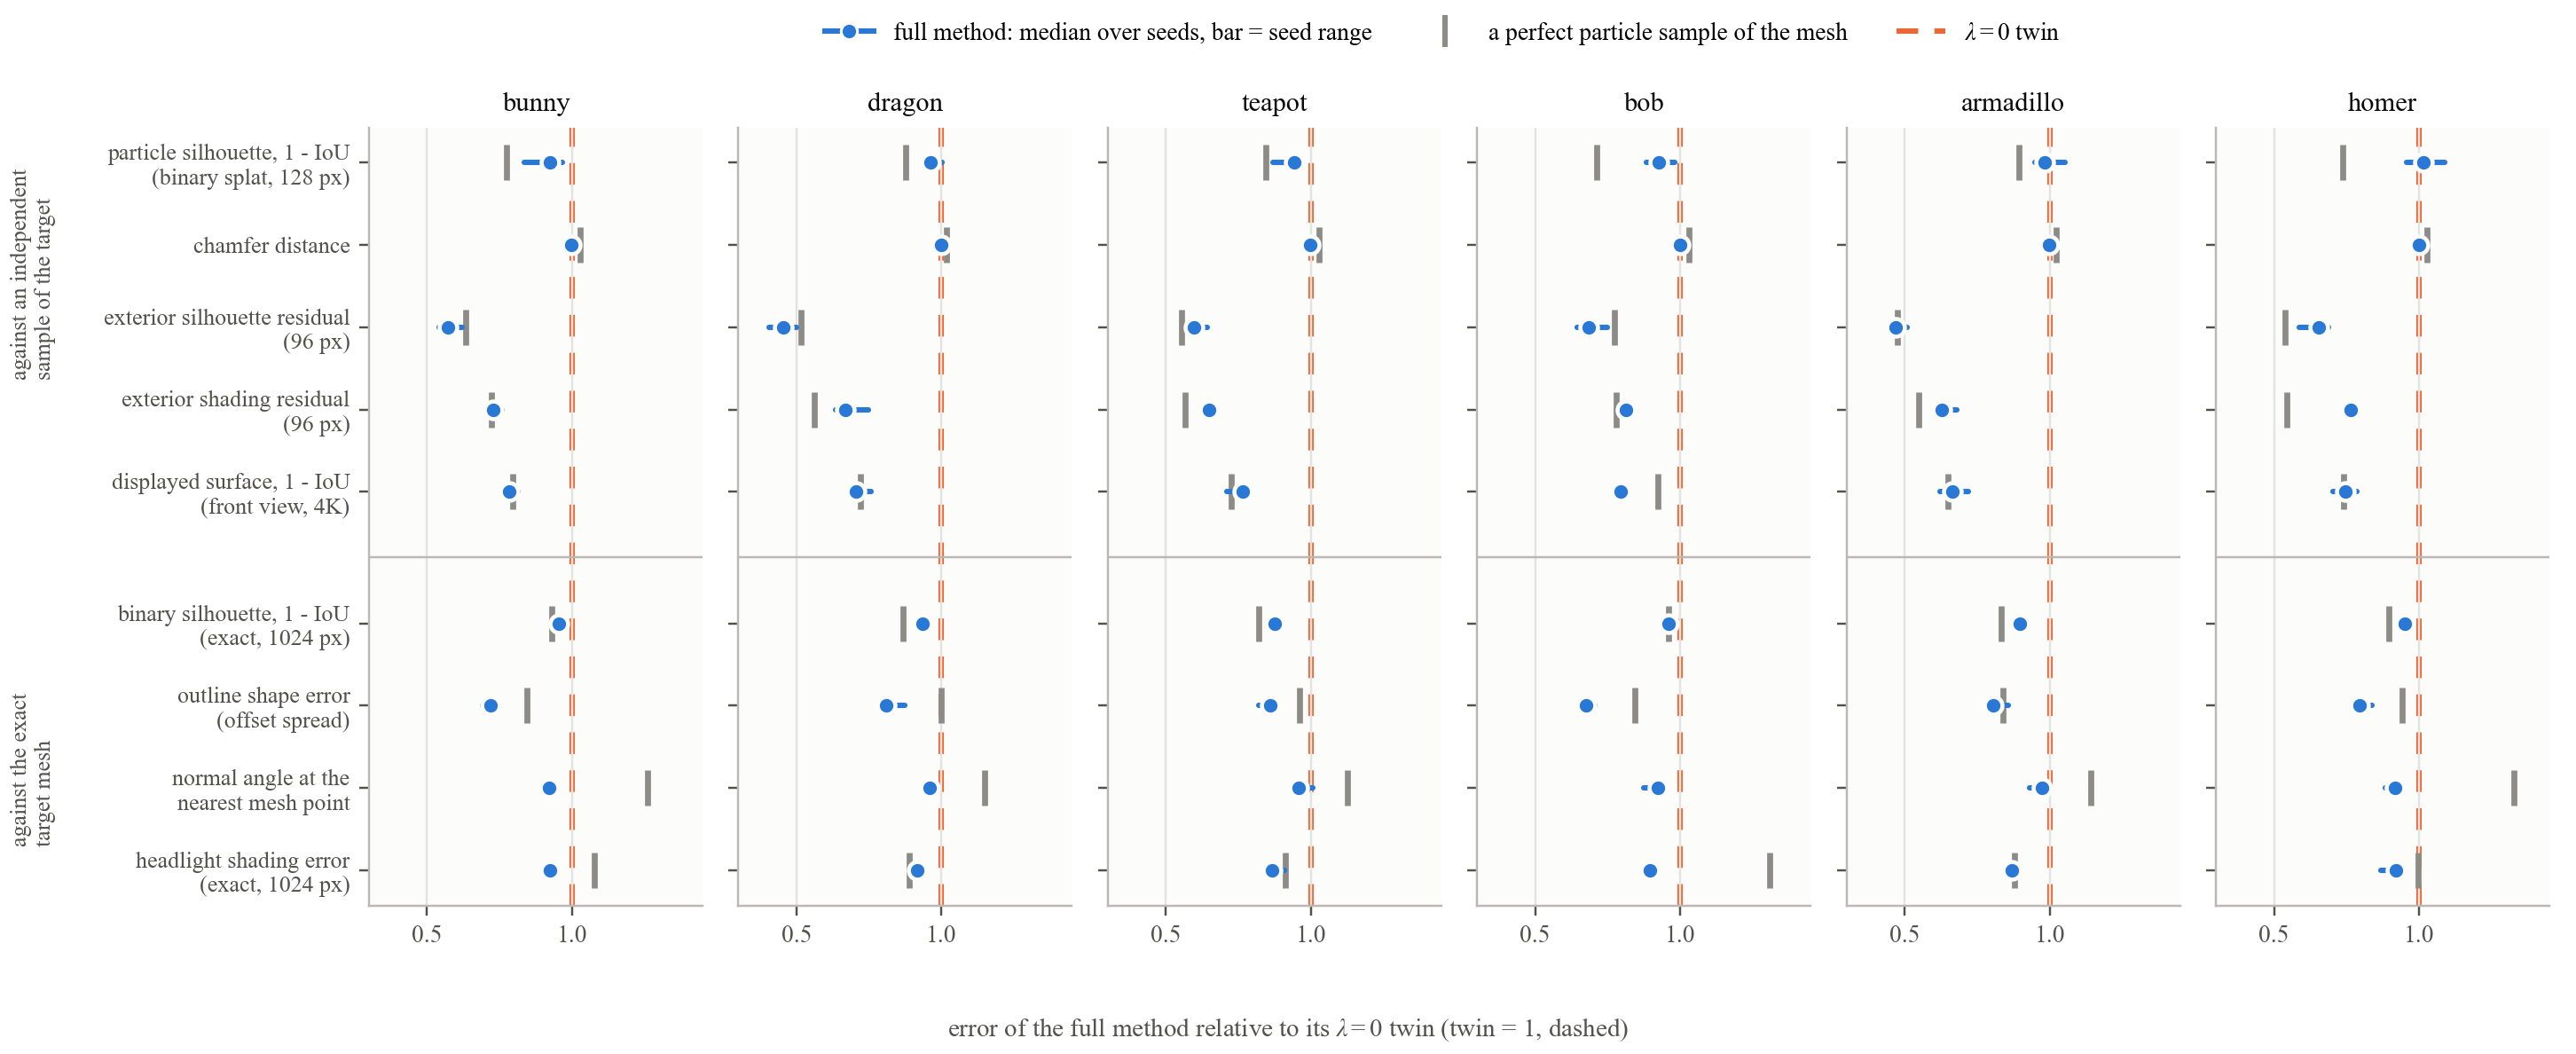
\includegraphics[width=\textwidth]{figs/ch4/fig_render_effect_end.png}
    \caption[{The end of the run, full method against its $\lambda=0$ twin on six meshes}]{\textbf{The end of the run, full method against its $\lambda=0$ twin on six meshes.} The render terms' own
    residuals move the most, the exact-mesh readings less, and the particle IoU and chamfer hardly at all.}
    \label{ch4:fig_render_end}
\end{figure*}

\textit{The particle silhouette.} The binary particle silhouette resolves about 1.8 pitches per pixel at 128\,px, and 72--89\,\%
of the twin's error there is the sampling floor itself. Moving the full method's outer layer uniformly by 0.1 pitch along its
normal changes $1-\mathrm{IoU}$ by 0.0008--0.0025, as much as the render term's whole effect, 0.0005--0.0021
(Figure~\ref{ch4:fig_iou}). Against the raw mesh, 78--80\,\% of the exact mask-IoU error at 300k is the exterior's shared offset.

\begin{figure}[t]
    \centering
    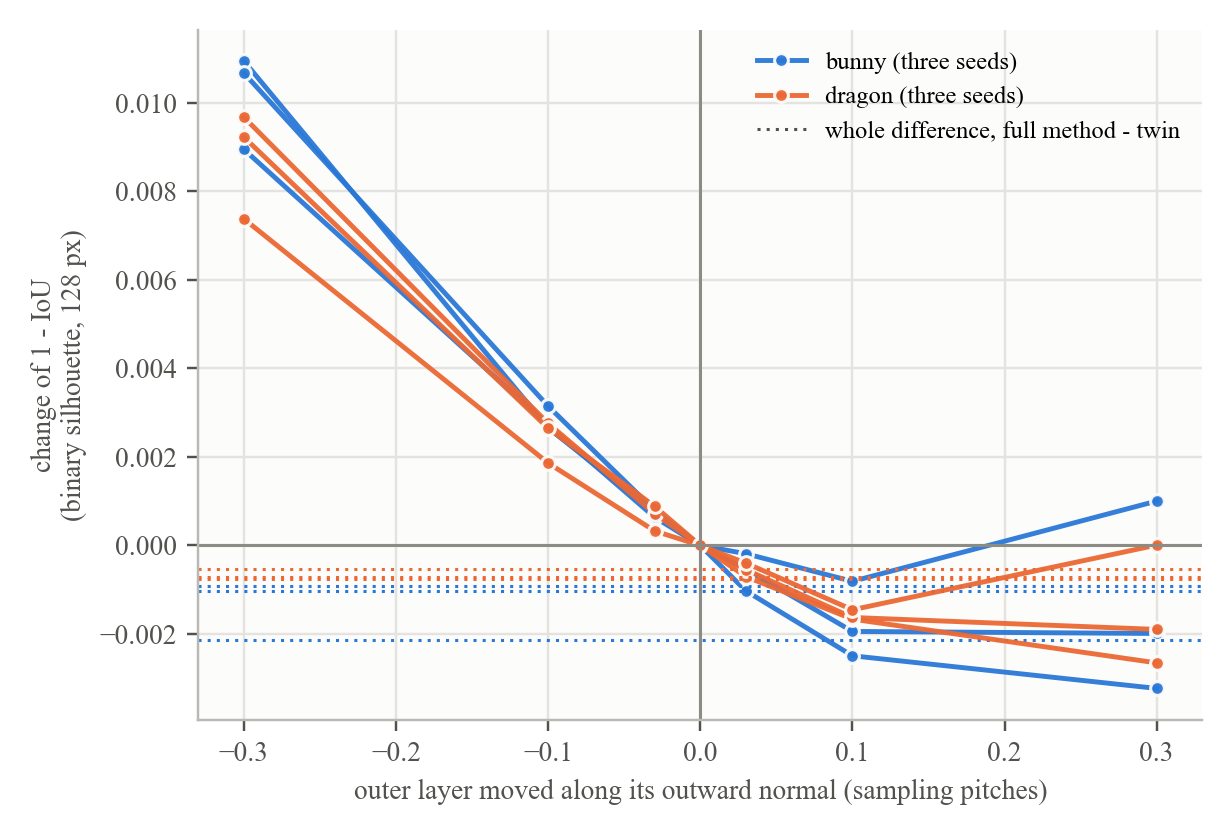
\includegraphics[width=0.62\linewidth]{figs/ch4/fig_iou_sensitivity.png}
    \caption[{Sensitivity of the particle silhouette IoU}]{\textbf{Sensitivity of the particle silhouette IoU.} A uniform shift of a tenth of a pitch moves it as much as the
    render term's entire effect (dotted).}
    \label{ch4:fig_iou}
\end{figure}

\textit{Arrangement.} Read on the run's own target pictures, the full method's render term at the end of the 300k runs is lower
than that of each of eight uniform samples of the true mesh on all five seeds of the bunny and the dragon: 0.46--0.58 (bunny)
and 0.69--0.79 (dragon) times their mean, against 1.4--1.9 times for the twin. The part of the full method's lead below that
floor is 43--56\,\% on the bunny and 21--26\,\% on the dragon, mostly in the silhouette term.

\subsection{The 40k Gallery}
\label{app:ch4_gallery}
On 19 meshes at three seeds, the full method's particle silhouette IoU is above its twin's at the three-seed mean on 18 of 19
meshes (bob is level), with a paired Wilcoxon test over the meshes giving $p=1.1\times10^{-5}$ and a median gain of $+0.0007$.
Against the exact meshes the outline deviates 3--15\,\% less than the twin's on all 19 meshes (56 of 57 pairs; median $-10$\,\%,
Figure~\ref{ch4:fig_g40}), and the normals come about 2\,\% closer; the binary silhouette error against the raw mesh is about
1\,\% higher, because the exterior sits 0.006 pitch farther out.

The lean comes from the silhouette term's 2:1 weighting. The target pictures' edge is 0.44--0.50 pitch wide for the eight-draw
mean against 0.27--0.33 for one draw; the asymmetry shifts the term's optimum outward on every state read (81 of 81 at 40k, 48 of
48 at 300k) by an amount set by the pitch, not the pixel. At 300k the twin's exterior lies outside the target pictures and the
term's net demand is inward, $-0.037$ pitch, which the full method follows (22 of 22 pairs); at 40k the twin sits near the
symmetric optimum ($+0.005$), and the full method's outline moves out by $+0.008$ pitch within a tenth of a render pixel of a
training outline (43 of 57 pairs, $p=2.8\times10^{-5}$), about a fifth of the term's uniform optimum, following the twin's demand
across mesh-seeds (Spearman 0.55). The pre-registered rule leaves the explanation undecided because the rim-against-head-on
contrast reached $p=0.020$; the next measurement is the gallery with equal weights.

\begin{figure}[t]
    \centering
    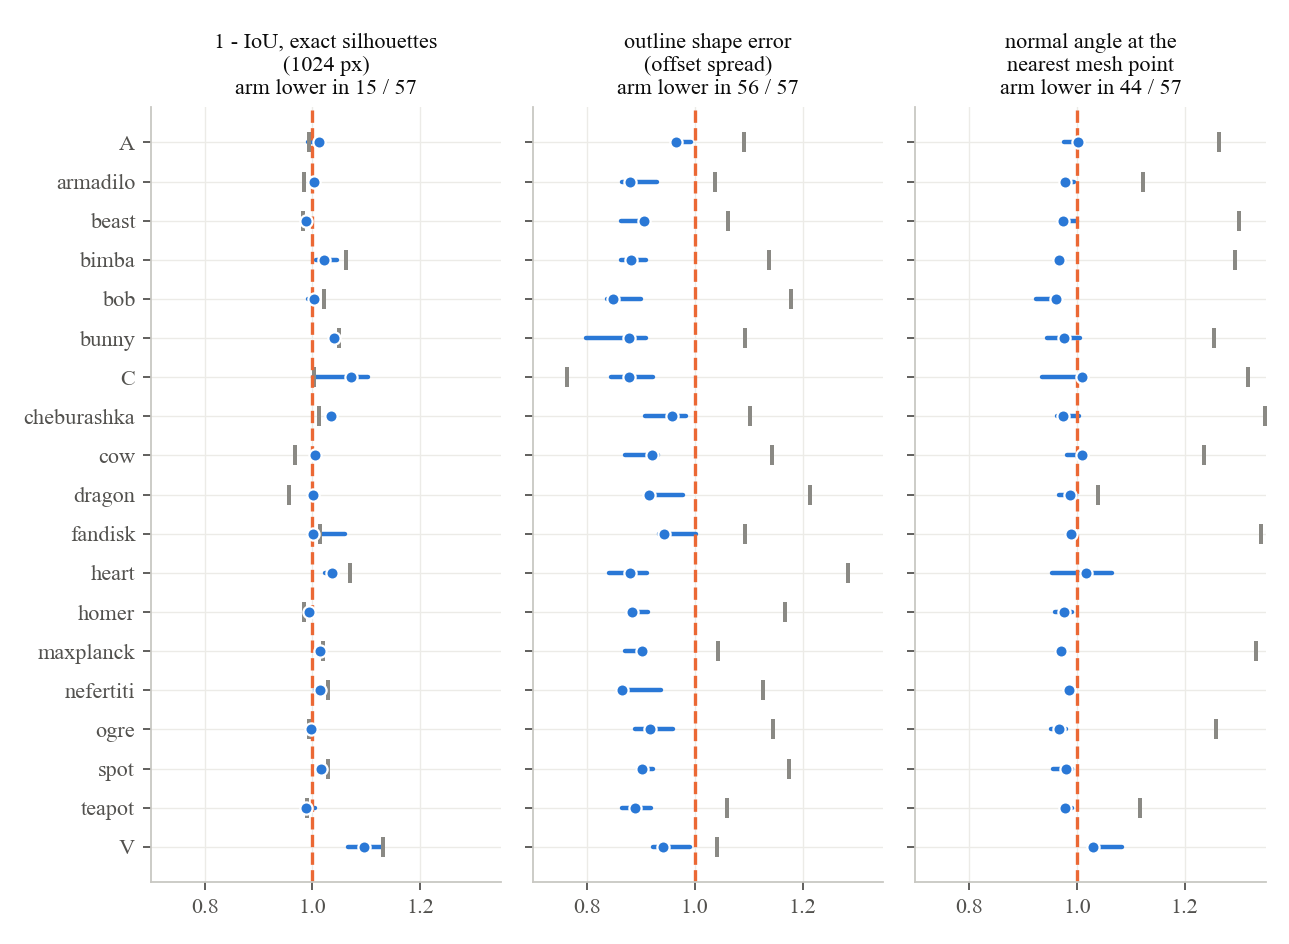
\includegraphics[width=0.85\linewidth]{figs/ch4/fig_gallery40k_mesh.png}
    \caption[{The 40k gallery against the exact meshes}]{\textbf{The 40k gallery against the exact meshes, full method relative to its twin (``arm'' in the panels).} The outline improves on all 19 meshes; the silhouette's area does not.}
    \label{ch4:fig_g40}
\end{figure}

\subsection{The 300k Gallery}
Against an independent sample, the 13 new targets reached from a sphere other than the letter C end at a particle silhouette
IoU of 0.9838--0.9901 and the six shape pairs at 0.9832--0.9888; no run has a piece of ten or more particles five pitches from
the body at its end, and every end but the letter C's has an end kinetic measure of at most $1.3\times10^{-5}$. A run to a new
target takes 7.8--27.8\,min and a shape pair 12.3--32.4\,min. Where twins were run, the full method's particle silhouette
error is 2--8\,\% lower and its exterior silhouette residual 30--58\,\% lower. A voxel reading of the Happy Buddha's end counts
seven tunnels against the target's six, and bunny $\to$ Happy Buddha opens four of the six.

\subsection{Materials and Gravity}
\label{app:ch4_gravity}
Every material reaches its target at 300k (particle IoU 0.9863--0.9876): a soft solid ($E\times0.1$) with a transport energy at
2\,s 55--178 times the default's, a stiff one ($E\times7$) with 2.2--3.5 times the default's end kinetic measure, and
$\nu=0.45$ at a cost of 9--21\,\% on some surface and thin measures; the render's lead on the exterior silhouette is $-29$ to
$-57$\,\%. Under gravity (0.65 world units\,s$^{-2}$, $G=\rho gH/E\approx0.02$) the single-body path stops two of three bunny
seeds and the twin after seven windows, because the landing raises the selection merit by 7--9\,\%. Through the scene path with a
standing target, both meshes reach on three of three seeds (particle IoU 0.9866--0.9875 bunny, 0.9871--0.9879 dragon, against
0.9860--0.9891 and 0.9866--0.9887 without gravity), end within 0.08 and 0.19 pitches of the standing height, stand within
$0.41^\circ$ of upright, and show no horizontal drift. The render's lead holds (particle IoU $+0.0010$ / $+0.0025$, exterior
silhouette residual $-49$ / $-56$\,\% at seed 97). The sag of the first 1.5\,s (0.14\,wu bunny, 0.27\,wu dragon) is partly made
rest shape at each commit, because a window is far shorter than the elastic period, so material keeps circulating (a mean particle
move of 0.026--0.050 pitch per kept-frame pair at the end, against 0.0012--0.0029 without gravity).

\subsection{Ablations}
\begin{table}[t]
\centering
\footnotesize
\setlength{\tabcolsep}{4pt}
\caption[{Ablations at 300k (bunny / dragon, three seeds)}]{\textbf{Ablations at 300k (bunny / dragon, three seeds).} Changes against the full method; all with seed ranges
apart unless marked ``within''.}
\label{ch4:tab_ablation}
\begin{tabular}{>{\raggedright\arraybackslash}p{3.6cm}>{\raggedright\arraybackslash}p{9.8cm}}
\toprule
part switched off & what changes \\
\midrule
layer offset $u$ (render loss kept) & exterior silhouette $\times3.0$ / $\times7.7$, shading $\times2.2$ / $\times4.0$,
  displayed surface $\times2.0$ / $\times3.4$, thin $+26\,\%$ / $\times3.0$; never at rest (end kinetic $\times54$ /
  $\times53$); early floating particles $-99$ / $-98\,\%$ \\
relief reference of the relaxation & dragon: exterior silhouette $+16\,\%$, shading $+20\,\%$; bunny thin $-23\,\%$ \\
volume-conserving body & early floating particles $\times5.0$ / $\times3.4$, end kinetic $+79$ / $+69\,\%$, dragon
  rotation $\times2.0$; distant pieces of up to 42 particles; thin $-25$ / $-21\,\%$ \\
\quad carried volume alone & early floating particles $\times5.1$ / $\times3.5$ \\
\quad volumetric assimilation alone & not at rest: end kinetic $\times36$ / $\times23$ \\
\quad density match alone & within the full method's range \\
render on the exterior (read on the cloud instead) & exterior silhouette $+28$ / $+44\,\%$, shading $+21$ / $+19\,\%$,
  displayed surface $+27$ / $+20\,\%$; particle IoU and thin within \\
render weight set every window (a moving average instead) & render share 0.42--0.80 in early windows; end within the
  range but for small shading and thin changes \\
minimum spacing & surface roughness $\times2.1$, thin $\times2.9$ / $\times3.8$, exterior silhouette $+37$ / $+41\,\%$,
  visible pieces $\times6.9$ / $\times7.6$ \\
relaxation in the driven half only (every step instead) & late wobble returns ($\times2.1$ / $\times1.8$); thin $+14$ /
  $+30\,\%$; runs end sooner \\
carried moments of $u$ (fresh every window instead) & window-to-window reversal returns; visible pieces $\times2.0$ /
  $\times2.3$ \\
symmetric minimum-spacing pairs & bunny centre-of-mass drift returns ($\times3$); shape within a few per cent \\
MPM cell from the shape (following $N$ instead) & mixed: gaps open earlier and thin parts improve on some meshes; bob's
  exterior silhouette $+34\,\%$; rest mixed \\
\bottomrule
\end{tabular}
\end{table}
Table~\ref{ch4:tab_ablation} lists the ablations. At 40k the cloud read's particle IoU is ahead of the exterior read on 17 of 19
meshes, and the driven-only relaxation also improves the particle silhouette on 13 of 19, while the carried moments and the
symmetric spacing are neutral there. The choices against late motion lengthen the dragon's runs.

\subsection{Stress against Force Control}
The plain force moves the centre of mass by 0.1--2.9 pitches and turns the body by up to $3.9^\circ$, $10^3$--$10^4$ and
$10^2$--$10^3$ times the stress control, with 77--158 times its angular momentum. Both force arms end with 3.1--5.7 times
(plain) and 4.5--5.1 times (projected; bob 207 times) the stress control's geometry energy and 17--97\,\% more exterior
silhouette error, at the same render share, and the projected force morphs 1.6--2.4 times slower.

\subsection{Comparison with Other Methods}
\label{app:ch4_comparison}
The F-control of Chapter~\ref{CH3_SHAPEMORPHING} is reimplemented in our simulator and verified at the published scale
($N=11{,}160$: a loss reduction of $-97.9$\,\% against the published $-98.3$\,\%). The volume-preserving neural morph and NISE
run from the former's code with the authors' defaults, and ISD and 4Deform from the authors' code. Both methods are driven
by a correspondence term: ISD takes given sparse correspondences and 4Deform estimates its own with a matching module. A sphere
and a target have no meaningful correspondences, so the main arm sets the matching weight to zero and does not use 4Deform's
matching module, and a second arm supplies radial correspondences (each sphere sample paired with the ray hit from the pair's
centre) on the bunny and the dragon. ARAP interpolation~\citep{2000-ARAPShapeInterpolation} runs in gradient-domain form~\citep{sumner2004deftransfer,2005-PoissonShapeInterpolation} with
the sphere correspondence from conformalized mean curvature flow~\citep{kazhdan2012cmcf}, on genus-zero targets. Large Steps and
FlexiCubes run with our 18 views at 188\,px (a) and with 25 views at 512\,px (b). Mesh and SDF frames are sampled by our volume
sampler at 300k; thin coverage is read on one shared set of thin points per mesh.

\begin{table*}[t]
\centering
\footnotesize
\setlength{\tabcolsep}{3pt}
\caption[{Every method on the six 300k targets}]{\textbf{Every method on the six 300k targets.} Per mesh the median over seeds, then the range over the meshes the
method ran on; ``ours ahead'' counts the meshes on which our seed range lies above the method's.}
\label{ch4:tab_methods}
\resizebox{\textwidth}{!}{%
\begin{tabular}{lcccccccccc}
\toprule
method & meshes & silhouette IoU & $1-\mathrm{IoU}$ & chamfer & thin uncovered & ours ahead & end genus & volume over & frames with a piece & wall \\
 & & (indep.) & / floor & / floor & (\%) & (meshes) & = target & the frames & $\geq5$ pitches off & time \\
\midrule
ours & 6 & 0.9864--0.9899 & 1.1--1.3 & 0.97--0.98$^e$ & 4.1--6.1 & -- & 3 of 6$^f$ & 0.96--1.09 & 0--8\,\% & 8.8--33.7\,min \\
F-control (Ch.~\ref{CH3_SHAPEMORPHING}) & 6 & 0.9396--0.9754 & 2.2--7.4 & 1.03--2.20 & 30.2--48.4 & 6 of 6 & (particles) & 0.72--1.35 & 7--98\,\% & 2.3--6.8\,min \\
vol.-preserving neural morph & 6 & 0.9163--0.9688 & 3.8--9.2 & 1.05--1.66 & 29.8--45.1 & 6 of 6 & 0 of 4$^a$ & 0.73--1.47 & 0--71\,\% & 45--47\,min$^b$ \\
NISE & 6 & 0.9660--0.9830 & 1.9--3.0 & 1.01--1.02 & 20.1--35.2 & 6 of 6 & 3 of 3$^a$ & 0.67--1.01 & 0--24\,\% & 13\,min$^b$ \\
ISD & 6 & 0.9822--0.9901 & 1.2--1.6 & 1.00--1.01 & 12.2--18.1 & 3 of 6 & 5 of 6 & 0.00--5.09 & 5--38\,\% & 27--39\,min \\
ISD, radial corr. & 2 & 0.9816--0.9862 & 1.3--1.7 & 1.01 & 14.3--19.0 & 1 of 2 & 1 of 2 & 0.36--3.99 & -- & 27--34\,min \\
4Deform & 6 & 0.4955--0.7628 & 26--57 & 2.8--10.3 & 67.5--81.5 & 6 of 6 & 3 of 6$^c$ & 0.24--2.10 & 0--10\,\% & 68--138\,min \\
4Deform, radial corr. & 2 & 0.9329--0.9784 & 2.0--6.0 & 1.04--3.94 & 22.7--32.2 & 2 of 2 & 0 of 2 & 0.86--1.48 & -- & 69--75\,min \\
ARAP$^d$ & 3 & 0.9849--0.9884 & 1.2--1.3 & 1.01 & 9.7--16.8 & 1 of 3 & 3 of 3 & 0.86--1.02 & 0\,\% & 0.2--12\,min \\
OT displacement & 2 & 0.9306--0.9440 & 5.0--6.5 & 1.04--1.11 & 24.0--24.7 & 2 of 2 & (particles) & 0.96--1.28 & 76--81\,\% & -- \\
Large Steps (a) & 6 & 0.9777--0.9881 & 1.2--2.0 & 1.01--1.46 & 9.7--17.7 & 3 of 6 & 3 of 6 & 0.85--1.74 & 0\,\% & 18--33\,s \\
Large Steps (b) & 6 & 0.9807--0.9897 & 1.2--2.1 & 1.01--1.17 & 9.6--16.3 & 3 of 6 & 3 of 6 & 0.84--1.62 & 0\,\% & 27--53\,s \\
FlexiCubes (a) & 6 & 0.8307--0.9315 & 7.5--20.7 & 1.21--6.64 & 53.5--70.8 & 6 of 6 & 0 of 6 & 0.76--1.10 & 67--86\,\% & 10--21\,s \\
FlexiCubes (b) & 6 & 0.9055--0.9803 & 2.2--11.6 & 1.02--3.61 & 31.2--60.8 & 6 of 6 & 0 of 6 & 0.73--1.20 & 57--90\,\% & 17--28\,s \\
\bottomrule
\end{tabular}}
\par\smallskip
\begin{minipage}{\textwidth}\scriptsize
$^a$Over the closed ends. $^b$Plus signed-distance fitting per shape. $^c$4Deform stays near the sphere.
$^d$Genus-zero targets only. $^e$Below the floor because our particles are more even than a random sample.
$^f$Our display surface, meshed: one watertight component without self-intersection in every frame read.
\end{minipage}
\end{table*}

\textit{The end.} Ours lies above every other method, with the seed ranges apart, on the dragon, the teapot and the armadillo,
and is level with ISD, Large Steps and ARAP on the bunny, bob and homer. On the shared thin points, ours leaves 4.1--6.1\,\%
uncovered, as many as a second sample of the mesh (2.9--8.1\,\%); every other method leaves at least 9.2\,\%. On the exterior
silhouette residual ours is ahead of every external method on five meshes (bunny $7.0$--$7.7\times10^{-4}$ against Large Steps
(b) at $10.0$--$12.0$ and ARAP at $10.7$) and level on the sixth. The F-control of Chapter~\ref{CH3_SHAPEMORPHING} ends with a
kinetic measure two to seven orders of magnitude above ours.

\textit{Against the exact mesh.} Read through our particle route, our held-out PSNR is the highest of every method on all six
meshes, and our Boundary IoU error is level with or below that of ISD and of Large Steps (b) on five of six. A perfect particle
sample read the same way has a lower Boundary IoU error than ours on four meshes and a higher F-score at half a pitch on five, but
a lower held-out PSNR on all six. Read on their own end meshes against the raw mesh, ISD and Large Steps (b) have a lower Boundary
IoU error than our route on three and four meshes; a perfect 300k particle sample trails them by a similar amount (on the bunny,
0.051--0.054 against Large Steps (b)'s 0.006--0.007).

\textit{Topology.} Our display surface, meshed by marching cubes~\citep{lorensen1998marching} and read by the mesh methods' readers, is one closed watertight
2-manifold without self-intersection at every frame read (22 ends, 18 mid-progress frames and 83 frames of the first seconds).
Its end genus matches the target on the bunny, bob and armadillo. The teapot's handle eye (about 5.5 pitches across, against an
MPM cell of 6.4 pitches) is filled, 13 of the dragon's 15 loops close, and the twin loses the same openings. With an MPM cell
that follows $N$ (3.3 pitches), the teapot's handle opens in both arms at 6.5--7\,s and the held-out Boundary IoU error falls by
17--36\,\% on the teapot, homer and the dragon, but the dragon opens only two or three of its loops, the early display is full of
holes (genus up to 92 on homer and 102 on the dragon at 1--2\,s), up to 155 particles leave the body beyond five pitches around
1.2--1.4\,s before rejoining by 2.6\,s, and the dragon's attempts take 2.3 times as long.

\textit{The way there.} In every ISD run the volume collapses in mid-run to 0.1--65\,\% of the target's, and 6--21 of its 21
frames have more than one component. Large Steps never opens the dragon's handles, the teapot's handle or bob's ring and imitates
them with self-intersecting surfaces (31 of 36 ends). FlexiCubes ends at a spurious genus of 4--58 on targets of genus 0--15.
4Deform with its matching weight at zero ends at a silhouette IoU of 0.50--0.76. Transport alone and the F-control of
Chapter~\ref{CH3_SHAPEMORPHING} have pieces farther than five pitches in 76--81\,\% and 7--98\,\% of their frames. Ours has such
pieces in 0--8\,\% of its frames with at most 14 particles, and its common occupancy reads 0.96--1.09 over every frame.

\subsection{Thrown and Dropped Bodies}
In the delivered throw (2 $\times$ 150k particles, $E\times7$), the bodies first touch at 3.8\,s with the morph 43\,\% complete,
part at 5.7\,s with a restitution of 0.95, land at 8.95 and 10.95\,s and tumble by $68^\circ$ and $127^\circ$; each ends at a
silhouette IoU of 0.985 / 0.984 in its own frame, momentum is kept within $2.7\times10^{-4}$ in every phase, and the run takes
50.5\,min. The dropped bunny (300k) lands at 2.5--2.6\,s at a fifth of the wave speed; eight particles at an ear tip move two to
six spacings off between 2.9 and 5.2\,s and rejoin, and the run takes 9.7\,min.

\subsection{The Render with Its Weight Held}
\label{app:ch4_held}
These runs back Section~\ref{ch4:sec_write}. In each, $\lambda$ is set by Eq.~\eqref{ch4:eq_lambda} at the first window
and then held, or only the colour term's weight is held; everything else, including the cleanup at $w_c=0.2$, is the
pipeline of this chapter. Each is compared with its $\lambda=0$ twin and with the same scene under the rule.

\textit{Where the render acts} (bunny, 300k, seed 97). Held, $\lambda$ stays at 0.321; under the rule it falls to 0.059 by
window 5, 0.0030 by window 20 and 0.0014 after window 40. The render's share of the outer layer's pull, aggregated over
groups of windows, is 0.20, 0.15, 0.14, 0.18 and 0.23 under the rule (windows 2--5, 6--10, 11--20, 21--40, after 40) and
0.59, 0.78, 0.88, 0.89 and 0.90 held; the render changes the outer layer's control relative to the twin by 11--20\,\%
under the rule after arrival and by 80--97\,\% held. At the end, the kinetic energy is $1.1\times10^{-3}$ held against
$1.0\times10^{-6}$ under the rule, the uncovered thin target points 5.7\,\% against 4.1\,\%, the silhouette IoU 0.9872
against 0.9884, and the stop rule ends the held run at 7.8\,s (54 windows) against 13--17\,s. One seed was run held.

\textit{Relief that exists only in the pictures.} The plaque spans $217\times67\times35$ pitches at 300k; the letters are
1.5 pitches high with 4.5-pitch strokes, and each face is seen in 9 of the 18 views, 8 of them oblique. We read the relief
the particles carry by its amplitude and its correlation with the lettering; the lettered mesh, sampled at 300k, gives the
ceiling, 1.16--1.23 pitches at a correlation of 0.59--0.60. Held ($\lambda=1.34$), the full method carves 0.69 pitch
(58\,\% of the ceiling; 0.67 on SIGGRAPH, 0.74 on VANDERBILT) at a correlation of 0.50, and its shading error on the
letter pixels is 40\,\% below the twin's; the twin carries $-0.05$. After the sixth window the render takes 94--99\,\% of
the step and pushes 40--100 times harder than the physics gradient. The cost: the end mean speed is 479 times the twin's,
the Chamfer distance to the smooth plaque rises by 0.09 pitch, the silhouette IoU falls from 0.9919 to 0.9851, the
uncovered thin points rise from 3.2 to 11\,\%, and the run stops at 4.0\,s after three rejected candidates (24 windows,
6\,min, against the twin's 112 windows and 23\,min); the held-out silhouette and the pieces are unchanged (no piece of 10 or
more particles). At 40k, the held run carves 91\,\% of its ceiling, while the rule leaves the plaque at the twin's level
(0.26 of the ceiling, the 40k reading's own floor being 0.21--0.27). The 300k run under the rule did not finish: another
user's job took its card after about 160 windows, by which point $\lambda$ had fallen to 1/4800 of its first value. On a
coin and a bunny lettered ``PM'' at 40k, the held weight carves 47--53\,\% and 54--58\,\% of the ceiling, from about one
second on, with end speeds 3--11 times the twin's.

\textit{Placement by appearance} (40k, seeds 97 and 99). The paint is checked to be invisible to the physics: with every
particle white, the run is bit for bit the run without colour, and the twin's trajectory is bit for bit the same under any
paint. Five scenes move the red material over a ladder of median distances: half (a control, 2.6 pitches), band (3.7),
ears (9.8), turn (12.4) and a dragon band (7.0). We report the recovered share $r$ of the twin's layout error (the share
of the exterior with the wrong colour). Under the rule $r=0.01$--$0.09$; with the whole render weight held,
$r=0.19$--$0.93$; with only the colour term held and the shape render terms under the rule, $r=0.67$--$1.00$, with the
turn at 0.75 and 0.69, and the held-out colour PSNR rises by 2.9--6.0\,dB. The cost of the colour-held runs: 12 of 80
shape cells fall short of the twin, mostly the F-score at half a pitch (by 0.001--0.002 on half and band, 0.01--0.07 on
turn and dragon); 7 of 10 runs miss the rest criterion fixed beforehand, by a factor of 1.1--4.2, exactly those whose
colour is still moving at the end; and on half, band and ears the surface sits 0.15--0.19 pitch rms from the twin's, since
the colour moves mostly by a circulation below the surface, red material sinking and white rising.

\textit{Which path carries the lettering} (40k, ``PM'' on a coin and a bunny, seeds 97 and 99, render weight held). With
$u$ switched off, the coin carves 0.18--0.19 of the ceiling against 0.47--0.53 with $u$, and the bunny 0.57--0.62 against
0.54--0.58; the twins stay at $-0.06$--$0.04$. Reading the physics placement terms only at the loss cell (the held render
with placement at the cell) carves 0.55--0.59 on the coin and 0.66--0.83 on the bunny. In every held arm the body is still
moving at the stop, at 3--49 times its twin's mean speed.

\textit{When the controls are released.} Released at the stop and left to settle, the held runs come to rest (mean speed
about $2\times10^{-5}$, below the twins' at their stop), the colour layout stays (band: $r$ 0.93--0.94 at the stop and
0.92--0.94 settled), and the carved relief falls to 0.17--0.29 of the ceiling from 0.56--0.75 at the stop, a third to two
fifths of it kept (0.29--0.43). Two mechanisms can remove it and have not yet been separated: the elastic part of the
stress the controls built up, and the outer-layer relaxation toward the smooth 3D target, which keeps acting in the
settling windows.

\textit{The press.} The finished plaque, letters down, is pressed into a slab of a twentieth of the base stiffness and lifted,
with the controls off; the plaque is made seven times stiffer than the base. At 300k the plaque keeps its end state, elastic
and plastic, and its print reaches a contrast of 0.13 particle spacings and a correlation of 0.46 with the letters, against
$-0.05$ and $-0.28$ for the twin with a decal. At 500k the end shape is taken as the rest shape; the plaque carries a
contrast of 0.68 spacings against the twin's 0.03, and its print, with the press's tilt and bend removed, correlates with
the letters at 0.65 against the twin's $-0.13$. At 40k the letters are shallower than the particle spacing, and the print
keeps only a band. In a still picture the twin's decal reads more crisply than the carving.

%% SWAP-IN: the settle and rest verdict (job 50), the stiffness (job 51), the 500k ripples and band (jobs 53/54) and the
% 300k ripples and band (job 55) go here when they land.

\subsection{Further Measured Costs}
\label{app:ch4_costs}
\textbf{Transient floaters.} The early arrival leaves a few particles apart from the body, mostly relief standing half a
pitch outside the displayed surface. None persists; on the display surface a few form separate specks of fewer than ten
particles, which the figures do not draw (Appendix~\ref{app:ch4_render}). Their main
source is $u$; a link that keeps each layer step near its neighbour removed most of them but moved the centre of mass, and
the next form makes that link symmetric, as the minimum spacing is.

\textbf{Angular momentum and the drag.} The ambient drag damps the particle momentum but not APIC's affine part. A drag that
damps the whole APIC momentum cut the largest angular momentum several-fold on a test body and kept shape and rest.

\textbf{A long, slow tail.} Most of the delivered frames come after the arrival. A target that moves along the transport's
displacement interpolation over the body's elastic period spreads the deformation in time, lowers the kinetic peak and the
early loose particles, keeps the render's lead, and ends at rest, but its end trails the fixed target's slightly on a few
meshes; the next measurement tells a shorter refit from under-supplied extremities.

\setlength{\emergencystretch}{1.5em}

% ============================================================================
% APPENDIX B: CulinaryCut / IntSim numerical implementation details
% ============================================================================
\clearpage
\chapter{IntSim Cutting Implementation Details}
\label{app:cutting-impl}

% Appendix A sets a fixed "A" equation prefix. Restore chapter-aware equation
% numbering for Appendix B without changing the preceding Appendix A.
\renewcommand{\theequation}{\thechapter.\arabic{equation}}
\setcounter{equation}{0}

This appendix records numerical details of IntSim's cutting resistance, damage thresholds, and time-step stabilization. These quantities are used inside the simulator and are not supplied as inputs to the evaluated VLA policies.

\section{Contact-Strength Normalization and Resistance Update}
\label{app:cut-contact-resistance}

A normalized contact-strength indicator $\hat c\in[0,1]$ is constructed using the characteristic speed $c_{\mathrm{norm}}=0.35\,\Delta x/\Delta t$. It gates blade-localized damage and modulates material-dependent resistance. With normalized speed $u=s/s_0$, the update is
\begin{equation}\label{eq:cut_resistance}
  u\leftarrow\frac{u}{1+k_2\,\hat c\,u\,\Delta t},
\end{equation}
where $k_2$ is scaled using properties such as Young's modulus $E$ and yield stress $\sigma_y$.

\section{Resolution-Dependent Damage Thresholds and Time-Step Constraint}
\label{app:cut-resolution-cfl}

Damage is gated by proximity to the blade SDF, contact strength, approach speed, and stroke direction as detailed in Chapter~\ref{CH5_CUTTINGSIM}. To adjust the band $|\phi|<b$ and the speed threshold across discretizations, the implementation uses
\begin{equation}\label{eq:cut_resolution_scaling}
  b=b_0\left(\frac{\Delta x_{\mathrm{ref}}}{\Delta x}\right)^\gamma,
  \qquad
  v_{\mathrm{th}}=\frac{\Delta x}{\Delta t}\,\hat v.
\end{equation}
Here $b_0$ and $\Delta x_{\mathrm{ref}}$ specify a reference band and grid spacing, while $\hat v$ is a dimensionless threshold. The exponent $\gamma$ is distinct from the morphing smoothing factor in Appendix~\ref{app:mlsmpm}.

With Lam\'e parameters $\lambda,\mu$ and material density $\rho$, explicit time stepping is constrained by
\begin{equation}\label{eq:cut_cfl}
  \Delta t\le 0.2\,\frac{\Delta x}{\sqrt{(\lambda+2\mu)/\rho}}.
\end{equation}
Additional numerical safeguards support robust rollouts but do not establish resolution-independent fracture accuracy.
